% Created by tikzDevice version 0.10.1 on 2018-02-17 17:07:06
% !TEX encoding = UTF-8 Unicode
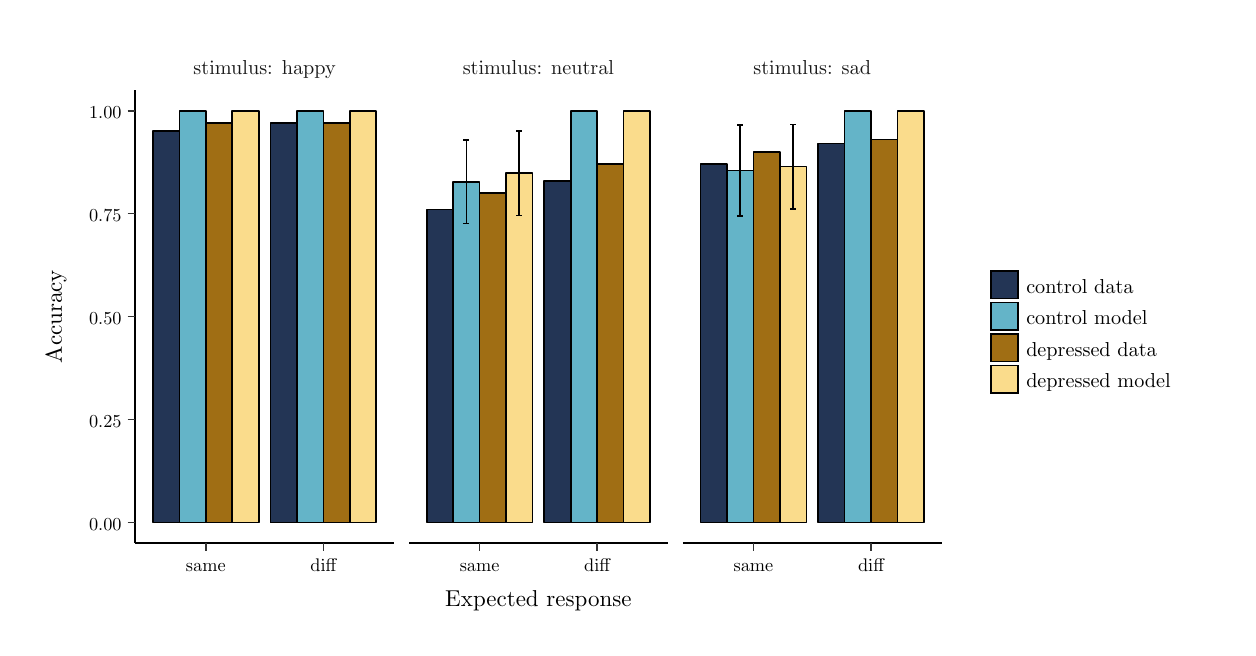
\begin{tikzpicture}[x=1pt,y=1pt]
\definecolor{fillColor}{RGB}{255,255,255}
\path[use as bounding box,fill=fillColor,fill opacity=0.00] (0,0) rectangle (433.62,216.81);
\begin{scope}
\path[clip] (  0.00,  0.00) rectangle (433.62,216.81);
\definecolor{drawColor}{RGB}{255,255,255}
\definecolor{fillColor}{RGB}{255,255,255}

\path[draw=drawColor,line width= 0.6pt,line join=round,line cap=round,fill=fillColor] (  0.00,  0.00) rectangle (433.62,216.81);
\end{scope}
\begin{scope}
\path[clip] ( 38.88, 30.56) rectangle (132.33,194.25);
\definecolor{fillColor}{RGB}{255,255,255}

\path[fill=fillColor] ( 38.88, 30.56) rectangle (132.33,194.25);
\definecolor{drawColor}{RGB}{0,0,0}
\definecolor{fillColor}{RGB}{250,220,140}

\path[draw=drawColor,line width= 0.6pt,line join=round,fill=fillColor] ( 73.93, 38.00) rectangle ( 83.48,186.81);
\definecolor{fillColor}{RGB}{160,110,20}

\path[draw=drawColor,line width= 0.6pt,line join=round,fill=fillColor] ( 64.37, 38.00) rectangle ( 73.93,182.34);
\definecolor{fillColor}{RGB}{100,180,200}

\path[draw=drawColor,line width= 0.6pt,line join=round,fill=fillColor] ( 54.81, 38.00) rectangle ( 64.37,186.81);
\definecolor{fillColor}{RGB}{35,53,85}

\path[draw=drawColor,line width= 0.6pt,line join=round,fill=fillColor] ( 45.26, 38.00) rectangle ( 54.81,179.37);
\definecolor{fillColor}{RGB}{250,220,140}

\path[draw=drawColor,line width= 0.6pt,line join=round,fill=fillColor] (116.40, 38.00) rectangle (125.96,186.81);
\definecolor{fillColor}{RGB}{160,110,20}

\path[draw=drawColor,line width= 0.6pt,line join=round,fill=fillColor] (106.84, 38.00) rectangle (116.40,182.34);
\definecolor{fillColor}{RGB}{100,180,200}

\path[draw=drawColor,line width= 0.6pt,line join=round,fill=fillColor] ( 97.29, 38.00) rectangle (106.84,186.81);
\definecolor{fillColor}{RGB}{35,53,85}

\path[draw=drawColor,line width= 0.6pt,line join=round,fill=fillColor] ( 87.73, 38.00) rectangle ( 97.29,182.34);

\path[draw=drawColor,line width= 0.6pt,line join=round] ( 77.64,186.81) --
	( 79.77,186.81);

\path[draw=drawColor,line width= 0.6pt,line join=round] ( 78.70,186.81) --
	( 78.70,186.81);

\path[draw=drawColor,line width= 0.6pt,line join=round] ( 77.64,186.81) --
	( 79.77,186.81);

\path[draw=drawColor,line width= 0.6pt,line join=round] ( 58.53,186.81) --
	( 60.65,186.81);

\path[draw=drawColor,line width= 0.6pt,line join=round] ( 59.59,186.81) --
	( 59.59,186.81);

\path[draw=drawColor,line width= 0.6pt,line join=round] ( 58.53,186.81) --
	( 60.65,186.81);

\path[draw=drawColor,line width= 0.6pt,line join=round] (120.12,186.81) --
	(122.24,186.81);

\path[draw=drawColor,line width= 0.6pt,line join=round] (121.18,186.81) --
	(121.18,186.81);

\path[draw=drawColor,line width= 0.6pt,line join=round] (120.12,186.81) --
	(122.24,186.81);

\path[draw=drawColor,line width= 0.6pt,line join=round] (101.00,186.81) --
	(103.13,186.81);

\path[draw=drawColor,line width= 0.6pt,line join=round] (102.07,186.81) --
	(102.07,186.81);

\path[draw=drawColor,line width= 0.6pt,line join=round] (101.00,186.81) --
	(103.13,186.81);
\end{scope}
\begin{scope}
\path[clip] (137.83, 30.56) rectangle (231.27,194.25);
\definecolor{fillColor}{RGB}{255,255,255}

\path[fill=fillColor] (137.83, 30.56) rectangle (231.27,194.25);
\definecolor{drawColor}{RGB}{0,0,0}
\definecolor{fillColor}{RGB}{250,220,140}

\path[draw=drawColor,line width= 0.6pt,line join=round,fill=fillColor] (172.87, 38.00) rectangle (182.43,164.21);
\definecolor{fillColor}{RGB}{160,110,20}

\path[draw=drawColor,line width= 0.6pt,line join=round,fill=fillColor] (163.31, 38.00) rectangle (172.87,157.05);
\definecolor{fillColor}{RGB}{100,180,200}

\path[draw=drawColor,line width= 0.6pt,line join=round,fill=fillColor] (153.76, 38.00) rectangle (163.31,161.11);
\definecolor{fillColor}{RGB}{35,53,85}

\path[draw=drawColor,line width= 0.6pt,line join=round,fill=fillColor] (144.20, 38.00) rectangle (153.76,151.09);
\definecolor{fillColor}{RGB}{250,220,140}

\path[draw=drawColor,line width= 0.6pt,line join=round,fill=fillColor] (215.34, 38.00) rectangle (224.90,186.81);
\definecolor{fillColor}{RGB}{160,110,20}

\path[draw=drawColor,line width= 0.6pt,line join=round,fill=fillColor] (205.79, 38.00) rectangle (215.34,167.46);
\definecolor{fillColor}{RGB}{100,180,200}

\path[draw=drawColor,line width= 0.6pt,line join=round,fill=fillColor] (196.23, 38.00) rectangle (205.79,186.81);
\definecolor{fillColor}{RGB}{35,53,85}

\path[draw=drawColor,line width= 0.6pt,line join=round,fill=fillColor] (186.67, 38.00) rectangle (196.23,161.51);

\path[draw=drawColor,line width= 0.6pt,line join=round] (176.59,179.44) --
	(178.71,179.44);

\path[draw=drawColor,line width= 0.6pt,line join=round] (177.65,179.44) --
	(177.65,148.99);

\path[draw=drawColor,line width= 0.6pt,line join=round] (176.59,148.99) --
	(178.71,148.99);

\path[draw=drawColor,line width= 0.6pt,line join=round] (157.47,176.20) --
	(159.60,176.20);

\path[draw=drawColor,line width= 0.6pt,line join=round] (158.53,176.20) --
	(158.53,146.01);

\path[draw=drawColor,line width= 0.6pt,line join=round] (157.47,146.01) --
	(159.60,146.01);

\path[draw=drawColor,line width= 0.6pt,line join=round] (219.06,186.81) --
	(221.18,186.81);

\path[draw=drawColor,line width= 0.6pt,line join=round] (220.12,186.81) --
	(220.12,186.81);

\path[draw=drawColor,line width= 0.6pt,line join=round] (219.06,186.81) --
	(221.18,186.81);

\path[draw=drawColor,line width= 0.6pt,line join=round] (199.95,186.81) --
	(202.07,186.81);

\path[draw=drawColor,line width= 0.6pt,line join=round] (201.01,186.81) --
	(201.01,186.81);

\path[draw=drawColor,line width= 0.6pt,line join=round] (199.95,186.81) --
	(202.07,186.81);
\end{scope}
\begin{scope}
\path[clip] (236.77, 30.56) rectangle (330.22,194.25);
\definecolor{fillColor}{RGB}{255,255,255}

\path[fill=fillColor] (236.77, 30.56) rectangle (330.22,194.25);
\definecolor{drawColor}{RGB}{0,0,0}
\definecolor{fillColor}{RGB}{250,220,140}

\path[draw=drawColor,line width= 0.6pt,line join=round,fill=fillColor] (271.81, 38.00) rectangle (281.37,166.62);
\definecolor{fillColor}{RGB}{160,110,20}

\path[draw=drawColor,line width= 0.6pt,line join=round,fill=fillColor] (262.26, 38.00) rectangle (271.81,171.93);
\definecolor{fillColor}{RGB}{100,180,200}

\path[draw=drawColor,line width= 0.6pt,line join=round,fill=fillColor] (252.70, 38.00) rectangle (262.26,165.20);
\definecolor{fillColor}{RGB}{35,53,85}

\path[draw=drawColor,line width= 0.6pt,line join=round,fill=fillColor] (243.14, 38.00) rectangle (252.70,167.46);
\definecolor{fillColor}{RGB}{250,220,140}

\path[draw=drawColor,line width= 0.6pt,line join=round,fill=fillColor] (314.29, 38.00) rectangle (323.85,186.81);
\definecolor{fillColor}{RGB}{160,110,20}

\path[draw=drawColor,line width= 0.6pt,line join=round,fill=fillColor] (304.73, 38.00) rectangle (314.29,176.39);
\definecolor{fillColor}{RGB}{100,180,200}

\path[draw=drawColor,line width= 0.6pt,line join=round,fill=fillColor] (295.18, 38.00) rectangle (304.73,186.81);
\definecolor{fillColor}{RGB}{35,53,85}

\path[draw=drawColor,line width= 0.6pt,line join=round,fill=fillColor] (285.62, 38.00) rectangle (295.18,174.90);

\path[draw=drawColor,line width= 0.6pt,line join=round] (275.53,181.85) --
	(277.65,181.85);

\path[draw=drawColor,line width= 0.6pt,line join=round] (276.59,181.85) --
	(276.59,151.38);

\path[draw=drawColor,line width= 0.6pt,line join=round] (275.53,151.38) --
	(277.65,151.38);

\path[draw=drawColor,line width= 0.6pt,line join=round] (256.42,181.58) --
	(258.54,181.58);

\path[draw=drawColor,line width= 0.6pt,line join=round] (257.48,181.58) --
	(257.48,148.82);

\path[draw=drawColor,line width= 0.6pt,line join=round] (256.42,148.82) --
	(258.54,148.82);

\path[draw=drawColor,line width= 0.6pt,line join=round] (318.01,186.81) --
	(320.13,186.81);

\path[draw=drawColor,line width= 0.6pt,line join=round] (319.07,186.81) --
	(319.07,186.81);

\path[draw=drawColor,line width= 0.6pt,line join=round] (318.01,186.81) --
	(320.13,186.81);

\path[draw=drawColor,line width= 0.6pt,line join=round] (298.89,186.81) --
	(301.02,186.81);

\path[draw=drawColor,line width= 0.6pt,line join=round] (299.95,186.81) --
	(299.95,186.81);

\path[draw=drawColor,line width= 0.6pt,line join=round] (298.89,186.81) --
	(301.02,186.81);
\end{scope}
\begin{scope}
\path[clip] ( 38.88,194.25) rectangle (132.33,211.31);
\definecolor{drawColor}{RGB}{255,255,255}
\definecolor{fillColor}{RGB}{255,255,255}

\path[draw=drawColor,line width= 1.1pt,line join=round,line cap=round,fill=fillColor] ( 38.88,194.25) rectangle (132.33,211.31);
\definecolor{drawColor}{gray}{0.10}

\node[text=drawColor,anchor=base,inner sep=0pt, outer sep=0pt, scale=  0.73] at ( 85.61,199.75) {stimulus: happy};
\end{scope}
\begin{scope}
\path[clip] (137.83,194.25) rectangle (231.27,211.31);
\definecolor{drawColor}{RGB}{255,255,255}
\definecolor{fillColor}{RGB}{255,255,255}

\path[draw=drawColor,line width= 1.1pt,line join=round,line cap=round,fill=fillColor] (137.83,194.25) rectangle (231.27,211.31);
\definecolor{drawColor}{gray}{0.10}

\node[text=drawColor,anchor=base,inner sep=0pt, outer sep=0pt, scale=  0.73] at (184.55,199.75) {stimulus: neutral};
\end{scope}
\begin{scope}
\path[clip] (236.77,194.25) rectangle (330.22,211.31);
\definecolor{drawColor}{RGB}{255,255,255}
\definecolor{fillColor}{RGB}{255,255,255}

\path[draw=drawColor,line width= 1.1pt,line join=round,line cap=round,fill=fillColor] (236.77,194.25) rectangle (330.22,211.31);
\definecolor{drawColor}{gray}{0.10}

\node[text=drawColor,anchor=base,inner sep=0pt, outer sep=0pt, scale=  0.73] at (283.49,199.75) {stimulus: sad};
\end{scope}
\begin{scope}
\path[clip] (  0.00,  0.00) rectangle (433.62,216.81);
\definecolor{drawColor}{RGB}{0,0,0}

\path[draw=drawColor,line width= 0.6pt,line join=round] ( 38.88, 30.56) --
	(132.33, 30.56);
\end{scope}
\begin{scope}
\path[clip] (  0.00,  0.00) rectangle (433.62,216.81);
\definecolor{drawColor}{gray}{0.20}

\path[draw=drawColor,line width= 0.6pt,line join=round] ( 64.37, 27.81) --
	( 64.37, 30.56);

\path[draw=drawColor,line width= 0.6pt,line join=round] (106.84, 27.81) --
	(106.84, 30.56);
\end{scope}
\begin{scope}
\path[clip] (  0.00,  0.00) rectangle (433.62,216.81);
\definecolor{drawColor}{RGB}{0,0,0}

\node[text=drawColor,anchor=base,inner sep=0pt, outer sep=0pt, scale=  0.66] at ( 64.37, 20.15) {same};

\node[text=drawColor,anchor=base,inner sep=0pt, outer sep=0pt, scale=  0.66] at (106.84, 20.15) {diff};
\end{scope}
\begin{scope}
\path[clip] (  0.00,  0.00) rectangle (433.62,216.81);
\definecolor{drawColor}{RGB}{0,0,0}

\path[draw=drawColor,line width= 0.6pt,line join=round] (137.83, 30.56) --
	(231.27, 30.56);
\end{scope}
\begin{scope}
\path[clip] (  0.00,  0.00) rectangle (433.62,216.81);
\definecolor{drawColor}{gray}{0.20}

\path[draw=drawColor,line width= 0.6pt,line join=round] (163.31, 27.81) --
	(163.31, 30.56);

\path[draw=drawColor,line width= 0.6pt,line join=round] (205.79, 27.81) --
	(205.79, 30.56);
\end{scope}
\begin{scope}
\path[clip] (  0.00,  0.00) rectangle (433.62,216.81);
\definecolor{drawColor}{RGB}{0,0,0}

\node[text=drawColor,anchor=base,inner sep=0pt, outer sep=0pt, scale=  0.66] at (163.31, 20.15) {same};

\node[text=drawColor,anchor=base,inner sep=0pt, outer sep=0pt, scale=  0.66] at (205.79, 20.15) {diff};
\end{scope}
\begin{scope}
\path[clip] (  0.00,  0.00) rectangle (433.62,216.81);
\definecolor{drawColor}{RGB}{0,0,0}

\path[draw=drawColor,line width= 0.6pt,line join=round] (236.77, 30.56) --
	(330.22, 30.56);
\end{scope}
\begin{scope}
\path[clip] (  0.00,  0.00) rectangle (433.62,216.81);
\definecolor{drawColor}{gray}{0.20}

\path[draw=drawColor,line width= 0.6pt,line join=round] (262.26, 27.81) --
	(262.26, 30.56);

\path[draw=drawColor,line width= 0.6pt,line join=round] (304.73, 27.81) --
	(304.73, 30.56);
\end{scope}
\begin{scope}
\path[clip] (  0.00,  0.00) rectangle (433.62,216.81);
\definecolor{drawColor}{RGB}{0,0,0}

\node[text=drawColor,anchor=base,inner sep=0pt, outer sep=0pt, scale=  0.66] at (262.26, 20.15) {same};

\node[text=drawColor,anchor=base,inner sep=0pt, outer sep=0pt, scale=  0.66] at (304.73, 20.15) {diff};
\end{scope}
\begin{scope}
\path[clip] (  0.00,  0.00) rectangle (433.62,216.81);
\definecolor{drawColor}{RGB}{0,0,0}

\path[draw=drawColor,line width= 0.6pt,line join=round] ( 38.88, 30.56) --
	( 38.88,194.25);
\end{scope}
\begin{scope}
\path[clip] (  0.00,  0.00) rectangle (433.62,216.81);
\definecolor{drawColor}{RGB}{0,0,0}

\node[text=drawColor,anchor=base east,inner sep=0pt, outer sep=0pt, scale=  0.66] at ( 33.93, 35.27) {0.00};

\node[text=drawColor,anchor=base east,inner sep=0pt, outer sep=0pt, scale=  0.66] at ( 33.93, 72.47) {0.25};

\node[text=drawColor,anchor=base east,inner sep=0pt, outer sep=0pt, scale=  0.66] at ( 33.93,109.68) {0.50};

\node[text=drawColor,anchor=base east,inner sep=0pt, outer sep=0pt, scale=  0.66] at ( 33.93,146.88) {0.75};

\node[text=drawColor,anchor=base east,inner sep=0pt, outer sep=0pt, scale=  0.66] at ( 33.93,184.08) {1.00};
\end{scope}
\begin{scope}
\path[clip] (  0.00,  0.00) rectangle (433.62,216.81);
\definecolor{drawColor}{gray}{0.20}

\path[draw=drawColor,line width= 0.6pt,line join=round] ( 36.13, 38.00) --
	( 38.88, 38.00);

\path[draw=drawColor,line width= 0.6pt,line join=round] ( 36.13, 75.20) --
	( 38.88, 75.20);

\path[draw=drawColor,line width= 0.6pt,line join=round] ( 36.13,112.40) --
	( 38.88,112.40);

\path[draw=drawColor,line width= 0.6pt,line join=round] ( 36.13,149.61) --
	( 38.88,149.61);

\path[draw=drawColor,line width= 0.6pt,line join=round] ( 36.13,186.81) --
	( 38.88,186.81);
\end{scope}
\begin{scope}
\path[clip] (  0.00,  0.00) rectangle (433.62,216.81);
\definecolor{drawColor}{RGB}{0,0,0}

\node[text=drawColor,anchor=base,inner sep=0pt, outer sep=0pt, scale=  0.83] at (184.55,  7.83) {Expected response};
\end{scope}
\begin{scope}
\path[clip] (  0.00,  0.00) rectangle (433.62,216.81);
\definecolor{drawColor}{RGB}{0,0,0}

\node[text=drawColor,rotate= 90.00,anchor=base,inner sep=0pt, outer sep=0pt, scale=  0.83] at ( 12.32,112.40) {Accuracy};
\end{scope}
\begin{scope}
\path[clip] (  0.00,  0.00) rectangle (433.62,216.81);
\definecolor{fillColor}{RGB}{255,255,255}

\path[fill=fillColor] (341.60, 78.37) rectangle (428.12,146.43);
\end{scope}
\begin{scope}
\path[clip] (  0.00,  0.00) rectangle (433.62,216.81);
\definecolor{drawColor}{RGB}{0,0,0}
\definecolor{fillColor}{RGB}{35,53,85}

\path[draw=drawColor,line width= 0.6pt,line cap=round,fill=fillColor] (348.00,118.92) rectangle (357.96,128.88);
\end{scope}
\begin{scope}
\path[clip] (  0.00,  0.00) rectangle (433.62,216.81);
\definecolor{drawColor}{RGB}{0,0,0}
\definecolor{fillColor}{RGB}{100,180,200}

\path[draw=drawColor,line width= 0.6pt,line cap=round,fill=fillColor] (348.00,107.54) rectangle (357.96,117.50);
\end{scope}
\begin{scope}
\path[clip] (  0.00,  0.00) rectangle (433.62,216.81);
\definecolor{drawColor}{RGB}{0,0,0}
\definecolor{fillColor}{RGB}{160,110,20}

\path[draw=drawColor,line width= 0.6pt,line cap=round,fill=fillColor] (348.00, 96.16) rectangle (357.96,106.11);
\end{scope}
\begin{scope}
\path[clip] (  0.00,  0.00) rectangle (433.62,216.81);
\definecolor{drawColor}{RGB}{0,0,0}
\definecolor{fillColor}{RGB}{250,220,140}

\path[draw=drawColor,line width= 0.6pt,line cap=round,fill=fillColor] (348.00, 84.77) rectangle (357.96, 94.73);
\end{scope}
\begin{scope}
\path[clip] (  0.00,  0.00) rectangle (433.62,216.81);
\definecolor{drawColor}{RGB}{0,0,0}

\node[text=drawColor,anchor=base west,inner sep=0pt, outer sep=0pt, scale=  0.73] at (360.84,120.87) {control data};
\end{scope}
\begin{scope}
\path[clip] (  0.00,  0.00) rectangle (433.62,216.81);
\definecolor{drawColor}{RGB}{0,0,0}

\node[text=drawColor,anchor=base west,inner sep=0pt, outer sep=0pt, scale=  0.73] at (360.84,109.49) {control model};
\end{scope}
\begin{scope}
\path[clip] (  0.00,  0.00) rectangle (433.62,216.81);
\definecolor{drawColor}{RGB}{0,0,0}

\node[text=drawColor,anchor=base west,inner sep=0pt, outer sep=0pt, scale=  0.73] at (360.84, 98.10) {depressed data};
\end{scope}
\begin{scope}
\path[clip] (  0.00,  0.00) rectangle (433.62,216.81);
\definecolor{drawColor}{RGB}{0,0,0}

\node[text=drawColor,anchor=base west,inner sep=0pt, outer sep=0pt, scale=  0.73] at (360.84, 86.72) {depressed model};
\end{scope}
\end{tikzpicture}
